%! Author = ia
%! Date = 4/22/22

% Preamble
\documentclass[11pt]{article}

% Packages
\usepackage{amsmath}

% Document
\begin{document}


%% %%%%%%%%%%%%%%%%%%%%%%%%%%%%%%%%%%%%%%%%%%%%%%%%%%%%%%%%%%%%%%%%%%%%%%%%%%%%%%%%%%%%%%%%%%%%%%%%%%%%%%%%%%

	\section{\normalsize{\textit{go-block-step}}}

	The program \texttt{main} in \textit{go-block-step/main.go} does not use
	a Poisson library or algorithm.
	Instead, mining is simulated.
	Search efficacy per miner is parameterized by network relative hashrate.
	The code relies on an arbitrary interval as the space from which a random needle
	is drawn. See code comments for more information.

	This coded model can be used to simulate network block emission, constant latency\nolinebreak
	\footnote{This is less of a concern than it may seem at first glance.}, and
	block authorship data.

	The model coded does not generate a blockchain. The model, instead,
	generates sample information for a single step (block increment)
	in the subtree, where the (assumed) parent block is held constant.
	Each sample is called a \texttt{round}.

%\begin{wrapfigure}{r}{0.3\textwidth}
	\begin{figure}[tph]
		\centering
		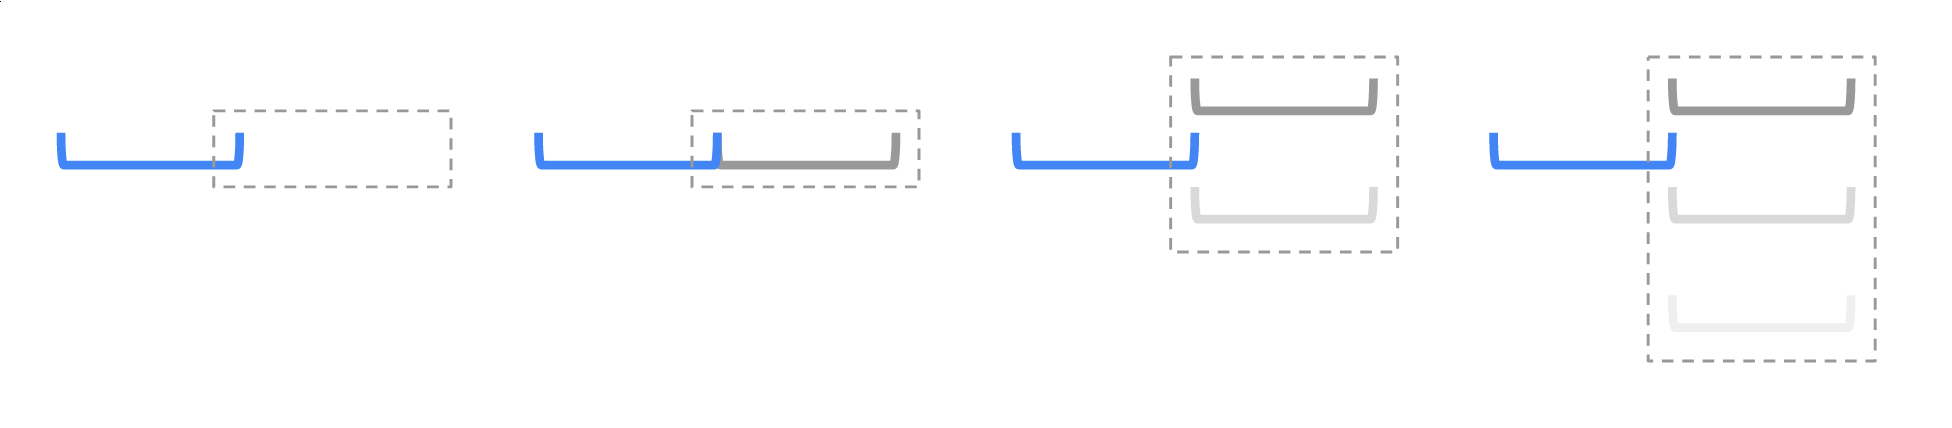
\includegraphics[height=3cm]{vis_theoretical_block-space.png}
		\caption{
			Visualizing theoretical outcomes for a block-space for some time interval
			$t$. The assumed existing parent block is blue.
		}
	\end{figure}

	For each round, the program is structured to assume a (any) sufficient $t$ such
	that at least one child block is produced. This $t$ value is pseudo-random, and
	is driven by the pseudo-randomness of the competing simulated miners.
	This $t$ value is recorded as, and here referred to, as the resulting
	\textit{interval} value.

	Notably, the model does not use $H_d$ (header difficulty) values.
	So long as we understand that the samples generated do not represent a continuous
	chain, we find that assuming a constant arbitrary $1$ value for the
	parent $TD$ value is reasonable.

	Our aim is to model block emissions in a pseudo-statistical way,
	focusing on game theoretical decisions for miners rather than
	block-network propagation or network shape.

	Latency is modeled only to the extent that it impacts block production
	intervals. A constant value is used; added to the recorded block interval
	for any miners who (probabilistically assigned) did not mine the
	parent block.

%This is, for example:
%
%  - Parent/Nothing \\ %% Blockchain turns off. Probably happens often.
%Unmeasured.
%  - Parent/Child \\
%  - Parent/Child,Child (twins/pending ommers|potential uncles,a fork,a
%bifurcation
%(of network consensus)) \\
%  - Parent/Child,Child,Child (triplets...a trifurcation (right!?))
%

%Another way to think of this is that the model replays the occurrence of the
%production of a single 'block-space' on the network (again, where the term
%block-space signals that zero \emph{or more} blocks could occupy the space (for some
%arbitrary interval unit, eg. $1$ second or $1$ milliscond, etc.). Necessary
%block values are held constant for an otherwise imaginary parent block.
%
%The aim of this paper intends specifically to deflect itself such as to entirely
%miss the mathematical aspects of graph theory or network algorithms, of which
%the author of this paragraph happens to have nearly exactly zero knowledge.

	We could introduce a small bit of randomness to the latency value, but that
	would only produce noise.

	We can play with latency. The program wants it to be understood as a tuneable
	parameter. For now, the program knows that same-author rounds add a latency of
	zero, while everyone else adds a constant legacy value
	\texttt{RoundConfiguration.Latency}, which is, as you guessed, configurable per
	round.

	We know that latency is an important thing.
	We assume, however, that the latency economy is efficient and nearly usally
	optimized,
	and that non-negligible-hashpower-share miners will be able to cost-effectively
	purchase sufficiently competitive latency values. With this, we assume that
	these same miners have approximately probably pretty much the same latencies.

	The model could be extended or modified to do latency differently.

	The model could also be changed to do hashrates and puzzle interval
	approximation differently.

	Implementation of a stateful block difficulty characteristics would enable
	representation of random walk information concerning network relative hashrates
	for miners. This would be more realistic, but would also be more noisy.



	The information generated is not deterministic.

	\textbf{Data}


	\begin{figure}[tph]
		\centering
		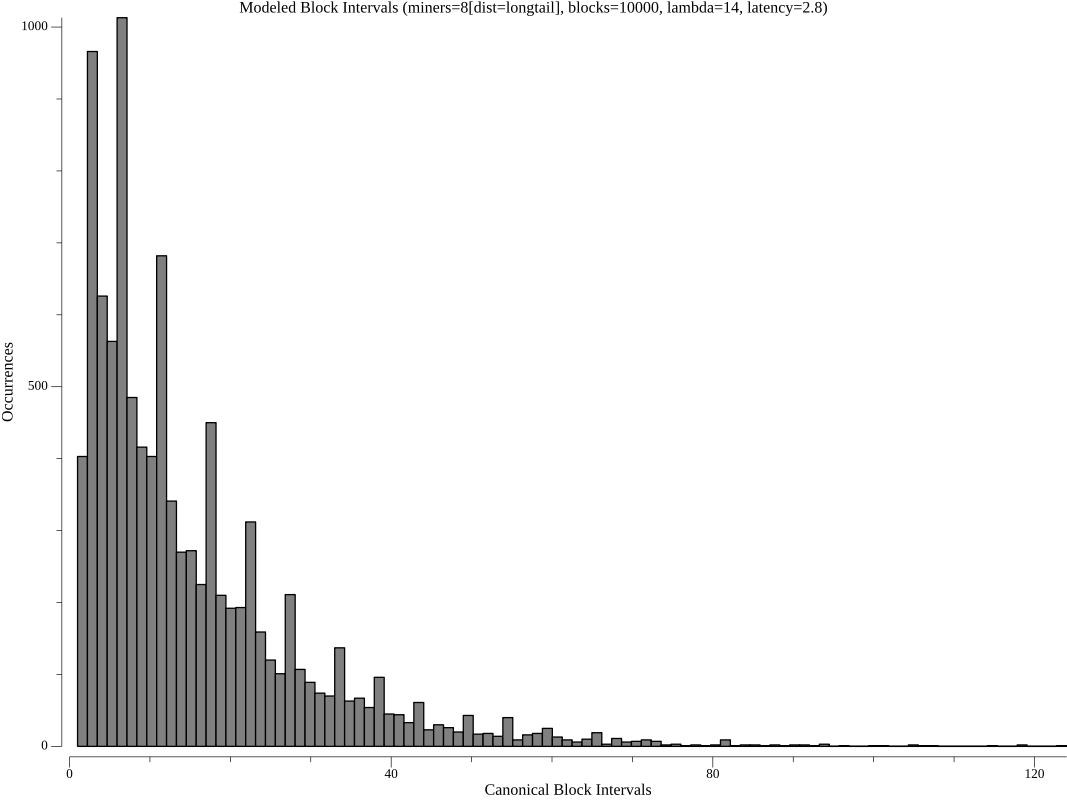
\includegraphics[width=1.0\textwidth]{go-poisson_A0_blockIntervals.png}
		\caption{
			Simulated block intervals for $\lambda=\frac{1}{14}$, $\eta=2.8$, with
			$8$ miners, each with procedurally generated long-tail-ish shaping
			relative hashrate shares.
		}
	\end{figure}

	\pagebreak

	The first \texttt{Round} generates a print out:

	\begin{verbatim}
CONFIG

Name:             A, ConsensusAlgorithm: TD,
NetworkLambda:    14, Latency:          2.80,
TickMultiple:     1, Rounds:           10000,
NumberOfMiners:   8, HashrateDistType: longtail,

GENERATED MINERS

Number: 8, Distribution: longtail, Hashrate Checksum OK:    true,
Hashrates: [0.333 0.222 0.148 0.099 0.066 0.059 0.044 0.02]

INTERVALS

Mean: 15.8650,
Med: 11.8000, Mode: [3.8000],
Min: 1.0000, Max: 139.8000,

ELIGIBLE AUTHORS PER BLOCK

Mean: 1.0819,
Med: 1.0000, Mode: [1.0000],
Min: 1.0000, Max: 3.0000,

MINER CANONICAL WINS

miner=0 hashrate=0.333 winrate=0.338 winrate/hashrate=1.013 (3375)
miner=1 hashrate=0.222 winrate=0.227 winrate/hashrate=1.020 (2266)
miner=2 hashrate=0.148 winrate=0.143 winrate/hashrate=0.963 (1427)
miner=3 hashrate=0.099 winrate=0.097 winrate/hashrate=0.979 (967)
miner=4 hashrate=0.066 winrate=0.066 winrate/hashrate=0.998 (657)
miner=5 hashrate=0.059 winrate=0.060 winrate/hashrate=1.022 (598)
miner=6 hashrate=0.044 winrate=0.043 winrate/hashrate=0.982 (431)
miner=7 hashrate=0.029 winrate=0.028 winrate/hashrate=0.953 (279)

	\end{verbatim}
	\pagebreak
	\begin{verbatim}

ANALYSIS

Ticks: 136550, Rounds (Blocks): 10000, Ticks/Block: 13.655
AuthorSameParentChildTally/Block: 0.211
ArbitrationDecisiveRate: 0.028, ArbitrationDecisiveTally: 277
ArbitrationIndecisiveRate: 0.052, ArbitrationIndecisiveTally: 522

	\end{verbatim}


	\section{\normalsize{Interlude: In Consideration of the Tick}}

	We have, until now, taken arbitrary rates, specifically \emph{rate units} for
	granted.

	Ethereum formally defines\footnote{Ethereum Yellow Paper} block timestamps as:

	\hypertarget{block_timestamp_H__s}{}$H_{\mathrm{s}}$ is the timestamp (in
	Unix's time()) of block $H$ and must fulfil the relation:
	\marginpar{Ethereum Yellow Paper}
	\begin{equation}
		H_{\mathrm{s}} > {P(H)_{\mathrm{H}}}_{\mathrm{s}}
	\end{equation}

	This mechanism enforces a homeostasis in terms of the time between blocks; a
	smaller period between the last two blocks results in an increase in the
	difficulty level and thus additional computation required, lengthening the
	likely next period. Conversely, if the period is too large, the difficulty, and
	expected time to the next block, is reduced.

	Timestamps are otherwise arbitrary.

	Time in the real world moves with apparently infinite fluidity. An instant of
	time is as small as the instance of a Cartesian point.

	Time in computers is as small as the time it takes for information to move.
	This is a bigger number than the theoretical instant.

	Time in Ethereum gets as small as $1$ second.
	The \texttt{go-ethereum} network client program \texttt{geth}\footnote{The
	majority share client on the Ethereum network}, ignores (does not process)
	blocks having a timestamp $B_s > now() + 15$. This is a normally undocumented
	subjective behavior, parameterized by some computer's clock. Running
	\texttt{geth} on a computer with a clock set 'late' (reading actually past
	values) will fail to maintain synchronisation (consensus) with the network.

	In coding a simulation, we can arbitrarily scale a \textit{tick} interval,
	representing some arbitrary atomic unit of time corresponding to a program step
	or loop. The tick parameterizes the time domain of the simulation.

	Since much of our work here assumes the job of fitting a model to the empirical
	information available, we need to acknowledge the limits of this approach.

	Our empirical knowledge is constrained (at this point in the research\footnote{
		For both practical and theoretical reasons.}) by using exlusively \emph{
		objective} measurements. Block timestamps are objective measurements.
	If we were to take our own readings of network latency, or of block production
	intervals (for example, by actually mining and recording measurements), these
	would be what this paper considers \emph{subjective} data.

	We do not consider any empirical information with time units less than $1$
	second. Our programming can be configured to represent a simulation of
	arbitrary time units. Evaluation of the degree of fit between model and
	data should take this into consideration.

\end{document}